
\chapter{Introduction \& Overview}
\label{sec:introduction}

The goal of this document is to describe the design and implementation of the Berkeley Out--of--Order Machine (BOOM). 


 BOOM is heavily inspired by the MIPS R10k and the Alpha 21264 out--of--order processors\cite{alpha21264, mipsr10k}.  Like the R10k and the 21264, BOOM is a unified physical register file design (also known as ``explicit register renaming"). 
 
 The source code to BOOM can be found at (\url{https://ucb-bar.github.io/riscv-boom}).

\section{The BOOM Pipeline}


\begin{figure}[ht]
	\centering
	\centerline{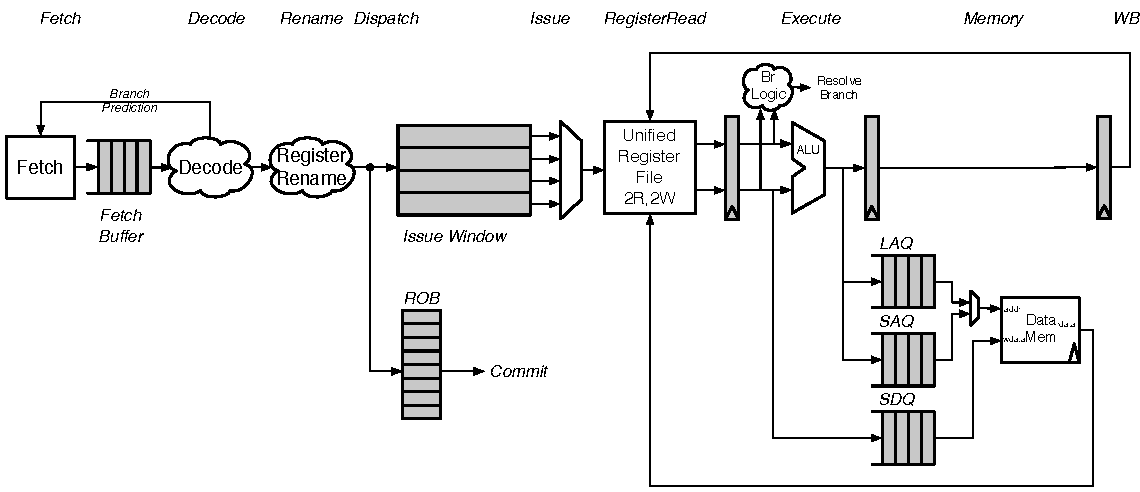
\includegraphics[scale =.9] {figures/boom_stages}}
	\caption{ \small The Berkeley Out of Order Machine Processor.}
	\label{fig:boom_stages}
\end{figure}



Conceptually, BOOM is broken up into 10 stages: {\em Fetch, Decode, Register Rename, Dispatch, Issue, Register Read, Execute, Memory, Writeback,} and {\em Commit}.  However, many of those stages are combined in the current implementation, yielding {\em six} stages: {\em Fetch, Decode/Rename/Dispatch, Issue/RegisterRead, Execute, Memory,} and {\em Writeback} ({\em Commit} occurs asynchronously, so I'm not counting that as part of the ``pipeline").   

\begin{quote}
\begin{description}
\item[Fetch]  Instructions are {\em fetched} from the Instruction Memory and placed into a four-entry deep FIFO, known as the {\em fetch buffer}.\footnote{While the fetch buffer is N-entries deep, it can instantly read out the first instruction on the front of the FIFO.  Put another way, instructions don't need to spend four cycles moving their way through the {\em fetch buffer} if there are no instructions in front of them.}
\item[Decode]
{\em Decode} pulls instructions out of the {\em fetch buffer} and generates the appropriate ``micro-op" to place into the pipeline.\footnote{Because RISC-V is a RISC ISA, currently all instructions generate only a single micro-op.} 

\item[Rename]
 The ISA, or ``logical", register specifiers are then {\em renamed} into ``physical" register specifiers.
  
\item[Dispatch] The instruction is then {\em dispatched}, or written, into the {\em Issue Window}.  
 
\item[Issue]   Instructions sitting in the {\em Issue Window} wait until all of their operands are ready, and are then {\em issued}.  This is the beginning of the out--of--order piece of the pipeline.
\item[RF Read]  Issued instructions first {\em read} their operands from the unified physical register file... 
\item[Execute] and then enter the {\em Execute} stage where the integer ALU resides.  Issued memory operations perform their address calculations in the {\em Execute} stage, and then store the calculated addresses in the Load/Store Unit which resides in the {\em Memory} stage.  
 
\item[Memory]  The Load/Store Unit consists of three queues: a Load Address Queue (LAQ), a Store Address Queue (SAQ), and a Store Data Queue (SDQ).  Loads are fired to memory when their address is present in the queue and does not conflict with any of the store addresses that the load depends on. Stores are fired to memory at commit time, when both its address and its data are present.  
 
\item[Writeback]  ALU operations and load operations are {\em written} back to the physical register file.
\item[Commit] The Reorder Buffer, or ROB, tracks the status of each instruction in the pipeline.  When the head of the ROB is not-busy, it {\em commits} the instruction.  For stores, the ROB signals to the store at the head of the Store Queue that it can now write its data to memory.
\end{description}
\end{quote}


  
BOOM supports full branch speculation and branch prediction.  Each instruction, no matter where it is in the pipeline,  is accompanied by a branch tag that marks which branches the instruction is ``speculated under". A mispredicted branch requires killing all instructions that depended on that branch.  When a branch instructions passes through {\em Rename}, copies of the {\em Register Rename Table} and the {\em Free List} are made.  On a mispredict, the saved processor state is restored.

Although Figure \ref{fig:boom_stages} shows a simplified pipeline, BOOM implements the RV64G and privileged ISAs, which includes single- and double-precision floating point, atomic memory support, and page-based virtual memory. 



\section{The RISC-V ISA}

BOOM implements the RV64G variant of the RISC-V ISA. This includes the MAFD
extensions and the privileged specification (multiply/divide, AMOs,
load-reserve/store-conditional, single- and double-precision IEEE
754-2008 floating point). More information about the RISC-V
ISA can be found at (\url{http://riscv.org}).

RISC-V provides the following features which make it easy to target with high-performance designs:

\begin{quote}
\begin{description}
\item [Relaxed memory model] This greatly simplifies the Load/Store Unit, which does not need to have loads snoop other loads nor does coherence traffic need to snoop the LSU, as required by sequential consistency.
\item [accrued floating point exception flags] The fp status register does not need to be renamed, nor can FP instructions throw exceptions themselves. 
\item [no integer side-effects] All integer ALU operations exhibit no side-effects, save the writing the destination register. This prevents the need to rename additional condition state.
\item [no \bf{cmov} or predication] Although predication can lower the branch predictor complexity of small designs, it greatly complicates OoO pipelines, including the addition of a third read port for integer operations.
\item [no implicit register specifiers] Even JAL requires specifying an explicit \tt{rd}. This simplifies rename logic, which prevents either the need to know the instruction first before accessing the rename tables, or it prevents adding more ports to remove the instruction decode off the critical path.
\item [\tt{rs1}, \tt{rs2}, \tt{rs3}, \tt{rd} are always in the same place] This allows decode and rename to proceed in parallel. 

\end{description}
\end{quote}

BOOM (currently) does not implement the ``C" compressed extension nor the ``V" vector extension.

\section{The \Chisel\ Hardware Construction Language}

BOOM is implemented in the \Chisel\ hardware construction language.  More information about \Chisel\ can be found at (\url{http://chisel.eecs.berkeley.edu}). 

\section{Quick-start}


To build a BOOM C++ emulator and run BOOM through a couple of simple tests:
\\

\texttt{\$} \verb=export ROCKETCHIP_ADDONS==\verb="boom"=

\texttt{\$} \verb=git clone https://github.com/ucb-bar/rocket-chip.git=

\texttt{\$} \verb=cd rocket-chip=

\texttt{\$} \verb=git checkout boom=

\texttt{\$} \verb=git submodule update --init=

\texttt{\$} \verb=cd riscv-tools=

\texttt{\$} \verb=git submodule update --init --recursive riscv-tests=

\texttt{\$} \verb=cd ../emulator; make run CONFIG==\verb=BOOMCPPConfig=


\section{The BOOM Repository}

The BOOM repository holds the source code to the BOOM core; it is not a full processor and thus is \textbf{NOT A SELF-RUNNING} repository.  To instantiate a BOOM core, the Rocket chip generator found in the rocket-chip git repository must be used (\url{https://github.com/ucb-bar/rocket-chip}), which provides the caches, uncore, and other needed infrastructure to support a full processor.

The BOOM source code can be found in \verb=boom/src/main/scala=.  

The code structure is shown below:

\begin{quote}
\begin{itemize}
\item \verb=boom/src/main/scala=/\begin{itemize}
  \item bpd\_pipeline.scala {\footnotesize \color{red} branch prediction stage.}
  \item brpredictor.scala {\footnotesize \color{red} abstract branch predictor.}
  \item configs.scala {\footnotesize \color{red} BOOM configurations. }
  \item consts.scala {\footnotesize \color{red} constant definitions. }
  \item core.scala {\footnotesize \color{red} the top-level of the processor core.}
  \item dcacheshim.scala {\footnotesize \color{red} the shim between the the core and the dcache.}
  \item decode.scala {\footnotesize \color{red} decode stage.}
  \item dpath.scala {\footnotesize \color{red} core datapath.}
  \item execute.scala {\footnotesize \color{red} high-level execution units (made up of FUs).}
  \item fpu.scala {\footnotesize \color{red} floating point unit.}
  \item functional\_unit.scala {\footnotesize \color{red} low-level functional units.}
  \item gshare.scala {\footnotesize \color{red} gshare branch predictor.}
  \item imul.scala {\footnotesize \color{red} integer multiplier.}
  \item issue\_ageordered.scala {\footnotesize \color{red} age-ordered (collasping-queue) issue window implementation.}
  \item issue.scala {\footnotesize \color{red} abstract issue window.}
  \item issue\_slot.scala {\footnotesize \color{red} An issue window slot.}
  \item issue\_unordered.scala {\footnotesize \color{red} un-ordered issue window implementation.}
  \item lsu.scala {\footnotesize \color{red} load/store unit.}
  \item package.scala {\footnotesize \color{red} }
  \item parameters.scala {\footnotesize \color{red} knobs/parameters.}
  \item prefetcher.scala {\footnotesize \color{red} data prefetcher.}
  \item regfile.scala {\footnotesize \color{red} register file.}
  \item registerread.scala {\footnotesize \color{red} registerRead stage and bypassing.}
  \item rename.scala {\footnotesize \color{red} register renaming logic.}
  \item rob.scala {\footnotesize \color{red} re-order buffer}
  \item tile.scala {\footnotesize \color{red} top-level tile.}
  \item util.scala {\footnotesize \color{red} utility code.}


\end{itemize}
\end{itemize}
\end{quote}




\section{The Rocket-chip Repository Layout}

As BOOM is just a core, an entire SoC infrastructure must be provided.  BOOM was developed to use the open-source Rocket-chip SoC generator (\url{https://github.com/ucb-bar/rocket-chip}). The Rocket-chip generator can instantiate a wide range of SoC designs, including cache-coherent multi-tile designs, cores with and without accelerators, and chips with or without a last-level shared cache. 




\begin{figure}[ht]
	\centering
	\centerline{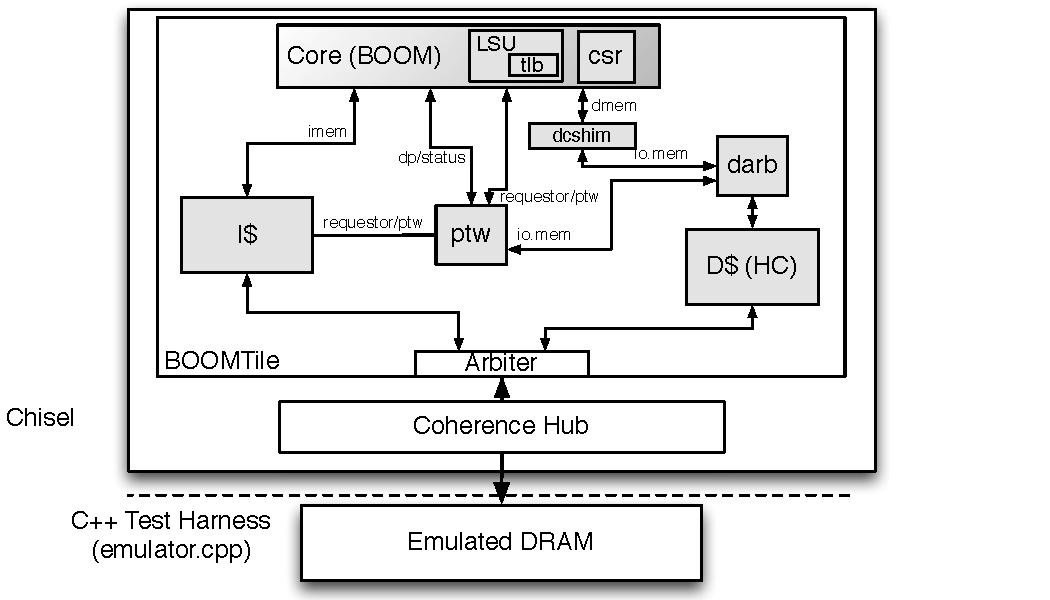
\includegraphics[scale =.9] {figures/chip}}
	\caption{ \small A single-core ``BOOM-chip", with no L2 last-level cache.}
	\label{fig:boomchip}
\end{figure}



To manage the wide array of actively developed projects that encompass Rocket-chip, the Rocket-chip repository makes heavy use of git submodules. The directory structure of the Rocket-chip repository is shown below. 

\begin{quote}
\begin{itemize}
\item \verb=${LAB3ROOT}=/\begin{itemize}

  \item boom/ {\footnotesize \color{red} Git submodule of the \Chisel\ source code for the BOOM core.}
  \item chisel {\footnotesize \color{red}  The source code to the {\tt Chisel} language itself.}
  
  \item emulator/ {\footnotesize \color{red} C++ simulation tools and support.}\begin{itemize}
    \item generated-src/{\footnotesize \color{red} Auto-generated C++ code.} 
    \item Makefile {\footnotesize \color{red} Makefile for C++ simulation.}
    \item output/{\footnotesize \color{red} Output files from C++ simulation runs.} 
    \end{itemize}
  \item junctions/ {\footnotesize \color{red} Git submodule of the \Chisel\ source code for the uncore and off-chip network.}
 \item riscv-tools/{\footnotesize \color{red} Git submodule that points to the RISC-V toolchain.}
 \begin{itemize} 
  \item riscv-tests/ {\footnotesize \color{red} Source code for benchmarks and tests.} \begin{itemize}
    \item riscv-bmarks/ {\footnotesize \color{red}  Benchmarks written in C.}
    \item riscv-tests/ {\footnotesize \color{red}  Tests written in assembly.}
  \end{itemize}
  \end{itemize}
   \item Makefrag {\footnotesize \color{red}  The high-level Makefile fragment.}
   
  \item src/ {\footnotesize \color{red} \Chisel\ source code for top-level Rocket-chip.}
  \item rocket/ {\footnotesize \color{red} Git submodule of the \Chisel\ source code for the Rocket core (used as a library of processor components).}
      \item sbt/ {\footnotesize \color{red} {\tt Chisel}/Scala voodoo.}
  \item uncore/ {\footnotesize \color{red} Git submodule of the \Chisel\ source code for the uncore components (including LLC).}
   
\end{itemize}
\end{itemize}
\end{quote}


